% -*- Mode:TeX -*-

%% IMPORTANT: The official thesis specifications are available at:
%%            http://libraries.mit.edu/archives/thesis-specs/
%%
%%            Please verify your thesis' formatting and copyright
%%            assignment before submission.  If you notice any
%%            discrepancies between these templates and the 
%%            MIT Libraries' specs, please let us know
%%            by e-mailing thesis@mit.edu

%% The documentclass options along with the pagestyle can be used to generate
%% a technical report, a draft copy, or a regular thesis.  You may need to
%% re-specify the pagestyle after you \include  cover.tex.  For more
%% information, see the first few lines of mitthesis.cls. 

%\documentclass[12pt,vi,twoside]{mitthesis}
%%
%%  If you want your thesis copyright to you instead of MIT, use the
%%  ``vi'' option, as above.
%%
%\documentclass[12pt,twoside,leftblank]{mitthesis}
%%
%% If you want blank pages before new chapters to be labelled ``This
%% Page Intentionally Left Blank'', use the ``leftblank'' option, as
%% above. 

\documentclass[12pt,twoside]{mitthesis}
\usepackage{lgrind}
%% These have been added at the request of the MIT Libraries, because
%% some PDF conversions mess up the ligatures.  -LB, 1/22/2014
\usepackage{cmap}
\usepackage[T1]{fontenc}
\pagestyle{plain}
\usepackage{xcolor}
\usepackage{booktabs}

\newcommand{\TODO}{\textcolor{red}{TODO}}

%% This bit allows you to either specify only the files which you wish to
%% process, or `all' to process all files which you \include.
%% Krishna Sethuraman (1990).

\begin{document}

% -*-latex-*-
% 
% For questions, comments, concerns or complaints:
% thesis@mit.edu
% 
%
% $Log: cover.tex,v $
% Revision 1.8  2008/05/13 15:02:15  jdreed
% Degree month is June, not May.  Added note about prevdegrees.
% Arthur Smith's title updated
%
% Revision 1.7  2001/02/08 18:53:16  boojum
% changed some \newpages to \cleardoublepages
%
% Revision 1.6  1999/10/21 14:49:31  boojum
% changed comment referring to documentstyle
%
% Revision 1.5  1999/10/21 14:39:04  boojum
% *** empty log message ***
%
% Revision 1.4  1997/04/18  17:54:10  othomas
% added page numbers on abstract and cover, and made 1 abstract
% page the default rather than 2.  (anne hunter tells me this
% is the new institute standard.)
%
% Revision 1.4  1997/04/18  17:54:10  othomas
% added page numbers on abstract and cover, and made 1 abstract
% page the default rather than 2.  (anne hunter tells me this
% is the new institute standard.)
%
% Revision 1.3  93/05/17  17:06:29  starflt
% Added acknowledgements section (suggested by tompalka)
% 
% Revision 1.2  92/04/22  13:13:13  epeisach
% Fixes for 1991 course 6 requirements
% Phrase "and to grant others the right to do so" has been added to 
% permission clause
% Second copy of abstract is not counted as separate pages so numbering works
% out
% 
% Revision 1.1  92/04/22  13:08:20  epeisach

% NOTE:
% These templates make an effort to conform to the MIT Thesis specifications,
% however the specifications can change.  We recommend that you verify the
% layout of your title page with your thesis advisor and/or the MIT 
% Libraries before printing your final copy.
\title{\TODO{} thesis title hi hi hi}

\author{Kimberli Zhong}
% If you wish to list your previous degrees on the cover page, use the 
% previous degrees command:
%       \prevdegrees{A.A., Harvard University (1985)}
% You can use the \\ command to list multiple previous degrees
%       \prevdegrees{B.S., University of California (1978) \\
%                    S.M., Massachusetts Institute of Technology (1981)}
\department{Department of Electrical Engineering and Computer Science}

% If the thesis is for two degrees simultaneously, list them both
% separated by \and like this:
% \degree{Doctor of Philosophy \and Master of Science}
\degree{Bachelor of Science in Computer Science and Engineering}

% As of the 2007-08 academic year, valid degree months are September, 
% February, or June.  The default is June.
\degreemonth{June}
\degreeyear{2018}
\thesisdate{May 25, 2018}

%% By default, the thesis will be copyrighted to MIT.  If you need to copyright
%% the thesis to yourself, just specify the `vi' documentclass option.  If for
%% some reason you want to exactly specify the copyright notice text, you can
%% use the \copyrightnoticetext command.  
%\copyrightnoticetext{\copyright IBM, 1990.  Do not open till Xmas.}

% If there is more than one supervisor, use the \supervisor command
% once for each.
\supervisor{William J. Dally}{Associate Professor}

% This is the department committee chairman, not the thesis committee
% chairman.  You should replace this with your Department's Committee
% Chairman.
\chairman{Arthur C. Smith}{Chairman, Department Committee on Graduate Theses}

% Make the titlepage based on the above information.  If you need
% something special and can't use the standard form, you can specify
% the exact text of the titlepage yourself.  Put it in a titlepage
% environment and leave blank lines where you want vertical space.
% The spaces will be adjusted to fill the entire page.  The dotted
% lines for the signatures are made with the \signature command.
\maketitle

% The abstractpage environment sets up everything on the page except
% the text itself.  The title and other header material are put at the
% top of the page, and the supervisors are listed at the bottom.  A
% new page is begun both before and after.  Of course, an abstract may
% be more than one page itself.  If you need more control over the
% format of the page, you can use the abstract environment, which puts
% the word "Abstract" at the beginning and single spaces its text.

%% You can either \input (*not* \include) your abstract file, or you can put
%% the text of the abstract directly between the \begin{abstractpage} and
%% \end{abstractpage} commands.

% First copy: start a new page, and save the page number.
\cleardoublepage{}
% Uncomment the next line if you do NOT want a page number on your
% abstract and acknowledgments pages.
% \pagestyle{empty}
\setcounter{savepage}{\thepage}
\begin{abstractpage}
Today, designers work in tandem with computerized tools to create stylized graphic designs, diagrams, and icons.
In this work, we explore the applications of generative modeling to the design of vectorized drawings, with a focus on font glyphs.
We establish a data-driven approach for creating preliminary graphics upon which designers can iterate.
To accomplish this, we present an end-to-end pipeline for a supervised training system on Scalable Vector Graphics (SVGs) that learns to reconstruct training data and produce similar but novel examples.
We demonstrate its results on selected characters using a Google Fonts dataset of 2552 font faces.
Our approach uses a variational autoencoder to learn sequences of SVG drawing commands and is capable of both recreating ground truth inputs and generating unseen, editable SVG outputs.
To investigate improvements to model performance, we perform two experiments: one on the effects of various SVG feature encodings on generated outputs, and one on a modified architecture that explicitly encodes style and class separately for multi-class generation.

\end{abstractpage}

% Additional copy: start a new page, and reset the page number.  This way,
% the second copy of the abstract is not counted as separate pages.
% Uncomment the next 6 lines if you need two copies of the abstract
% page.
% \setcounter{page}{\thesavepage}
% \begin{abstractpage}
% Today, designers work in tandem with computerized tools to create stylized graphic designs, diagrams, and icons.
In this work, we explore the applications of generative modeling to the design of vectorized drawings, with a focus on font glyphs.
We establish a data-driven approach for creating preliminary graphics upon which designers can iterate.
To accomplish this, we present an end-to-end pipeline for a supervised training system on Scalable Vector Graphics (SVGs) that learns to reconstruct training data and produce similar but novel examples.
We demonstrate its results on selected characters using a Google Fonts dataset of 2552 font faces.
Our approach uses a variational autoencoder to learn sequences of SVG drawing commands and is capable of both recreating ground truth inputs and generating unseen, editable SVG outputs.
To investigate improvements to model performance, we perform two experiments: one on the effects of various SVG feature encodings on generated outputs, and one on a modified architecture that explicitly encodes style and class separately for multi-class generation.

% \end{abstractpage}

\cleardoublepage{}

\section*{Acknowledgments}

This is the acknowledgements section.  You should replace this with your
own acknowledgements.

%%%%%%%%%%%%%%%%%%%%%%%%%%%%%%%%%%%%%%%%%%%%%%%%%%%%%%%%%%%%%%%%%%%%%%
% -*-latex-*-

% Some departments (e.g. 5) require an additional signature page.  See
% signature.tex for more information and uncomment the following line if
% applicable.
% % -*- Mode:TeX -*-
%
% Some departments (e.g. Chemistry) require an additional cover page
% with signatures of the thesis committee.  Please check with your
% thesis advisor or other appropriate person to determine if such a 
% page is required for your thesis.  
%
% If you choose not to use the "titlepage" environment, a \newpage
% commands, and several \vspace{\fill} commands may be necessary to
% achieve the required spacing.  The \signature command is defined in
% the "mitthesis" class
%
% The following sample appears courtesy of Ben Kaduk <kaduk@mit.edu> and
% was used in his June 2012 doctoral thesis in Chemistry. 

\begin{titlepage}
\begin{large}
This doctoral thesis has been examined by a Committee of the Department
of Chemistry as follows:

\signature{Professor Jianshu Cao}{Chairman, Thesis Committee \\
   Professor of Chemistry}

\signature{Professor Troy Van Voorhis}{Thesis Supervisor \\
   Associate Professor of Chemistry}

\signature{Professor Robert W. Field}{Member, Thesis Committee \\
   Haslam and Dewey Professor of Chemistry}
\end{large}
\end{titlepage}


\pagestyle{plain}
  % -*- Mode:TeX -*-
%% This file simply contains the commands that actually generate the table of
%% contents and lists of figures and tables.  You can omit any or all of
%% these files by simply taking out the appropriate command.  For more
%% information on these files, see appendix C.3.3 of the LaTeX manual. 
\tableofcontents
\newpage
\listoffigures
\newpage
\listoftables


\chapter{Introduction}

\TODO{hook}

Our motivation for examining the \textit{generation} of designs is two-fold.
One, we see practical purpose in a recommendation tool that augments a designer's experience, and we believe such a tool would be a valuable addition to a designer's creative process.
Two, we believe demystifying their generation would further solidify understanding of the intent and structure of human-created designs.
In algorithmically mimicking the process by which glyphs are created, we hope to gain a deeper grasp of from where humans' notion of design and style arises.

Although many strides have been made in understanding and synthesizing rasterized images and designs, primarily with convolutional neural networks, we focus our investigation on the domain of vectorized images in this work.
The two representations are quite different, and we aim to both produce generated designs with fewer aesthetically displeasing artifacts as well as investigate what new information about designs' underlying shapes and structures can be quantified and learned with the vectorized data format.

In the next chapter, we provide further background on the domain and discuss related work.
Then, in the following chapters, we delve into the methods used to train our vector graphics generator on the data processing side as well as the model architecture side.
We then demonstrate our methods as applied to font glyph generation, using a single-class as well as a multi-class approach.
Finally, we evaluate our results quantitatively and qualitatively and consider future directions of work.

% \chapter{Background}
The problem space we explore ties together work across a number of different disciplines, including graphics, graphic design, and machine learning modeling.
In applying generative methods to vectorized glyphs, we are inspired by previous work in computer vision on non-natural images and draw upon recent developments in the generative modeling of line drawings.

\section{Non-natural images}
While natural images are photographs of real-world scenes and objects, non-natural images are computationally generated, either by hand with a computer design tool or automatically.
Images in this category include graphs, pictograms, virtual scenes, graphic designs, and more.
Algorithmically understanding, summarizing, and synthesizing these images pose unique challenges because of the images' clean and deliberately drawn designs, amalgamation of distinct visual and textual elements, and purposeful or narrative nature.

While much attention has been focused on research problems like object recognition, scene segmentation, and classification on natural images, interest in applying computer vision methods to non-natural images has been growing.
Much progress has been made towards computationally understanding non-natural images on datasets including XML-encoded abstract scenes~\cite{wu2017neural}, comic strips~\cite{iyyer2016amazing}, and textbook diagrams~\cite{seo2014diagram}.
Recent work by our group has explored the space of infographics, complex diagrams composed of visual and textual elements that deliver a message~\cite{bylinskii2017understanding}.

\subsection{Font faces}
Within the space of non-natural images, we focus specifically on designer-crafted font faces.
Fonts are used to typeset text with particular styles and weights, and many types of fonts exist, including serif, sans serif, and handwriting style fonts (see Figure~\ref{fig:fonttypes}).
Each font is defined by a set of glyphs, which include letters, digits, symbols, and potentially other Unicode characters.
Within a font face, glyphs generally share the same style for properties like angles, curvature, presence of serifs, and stroke width.

\begin{figure}[h]
    \centering
	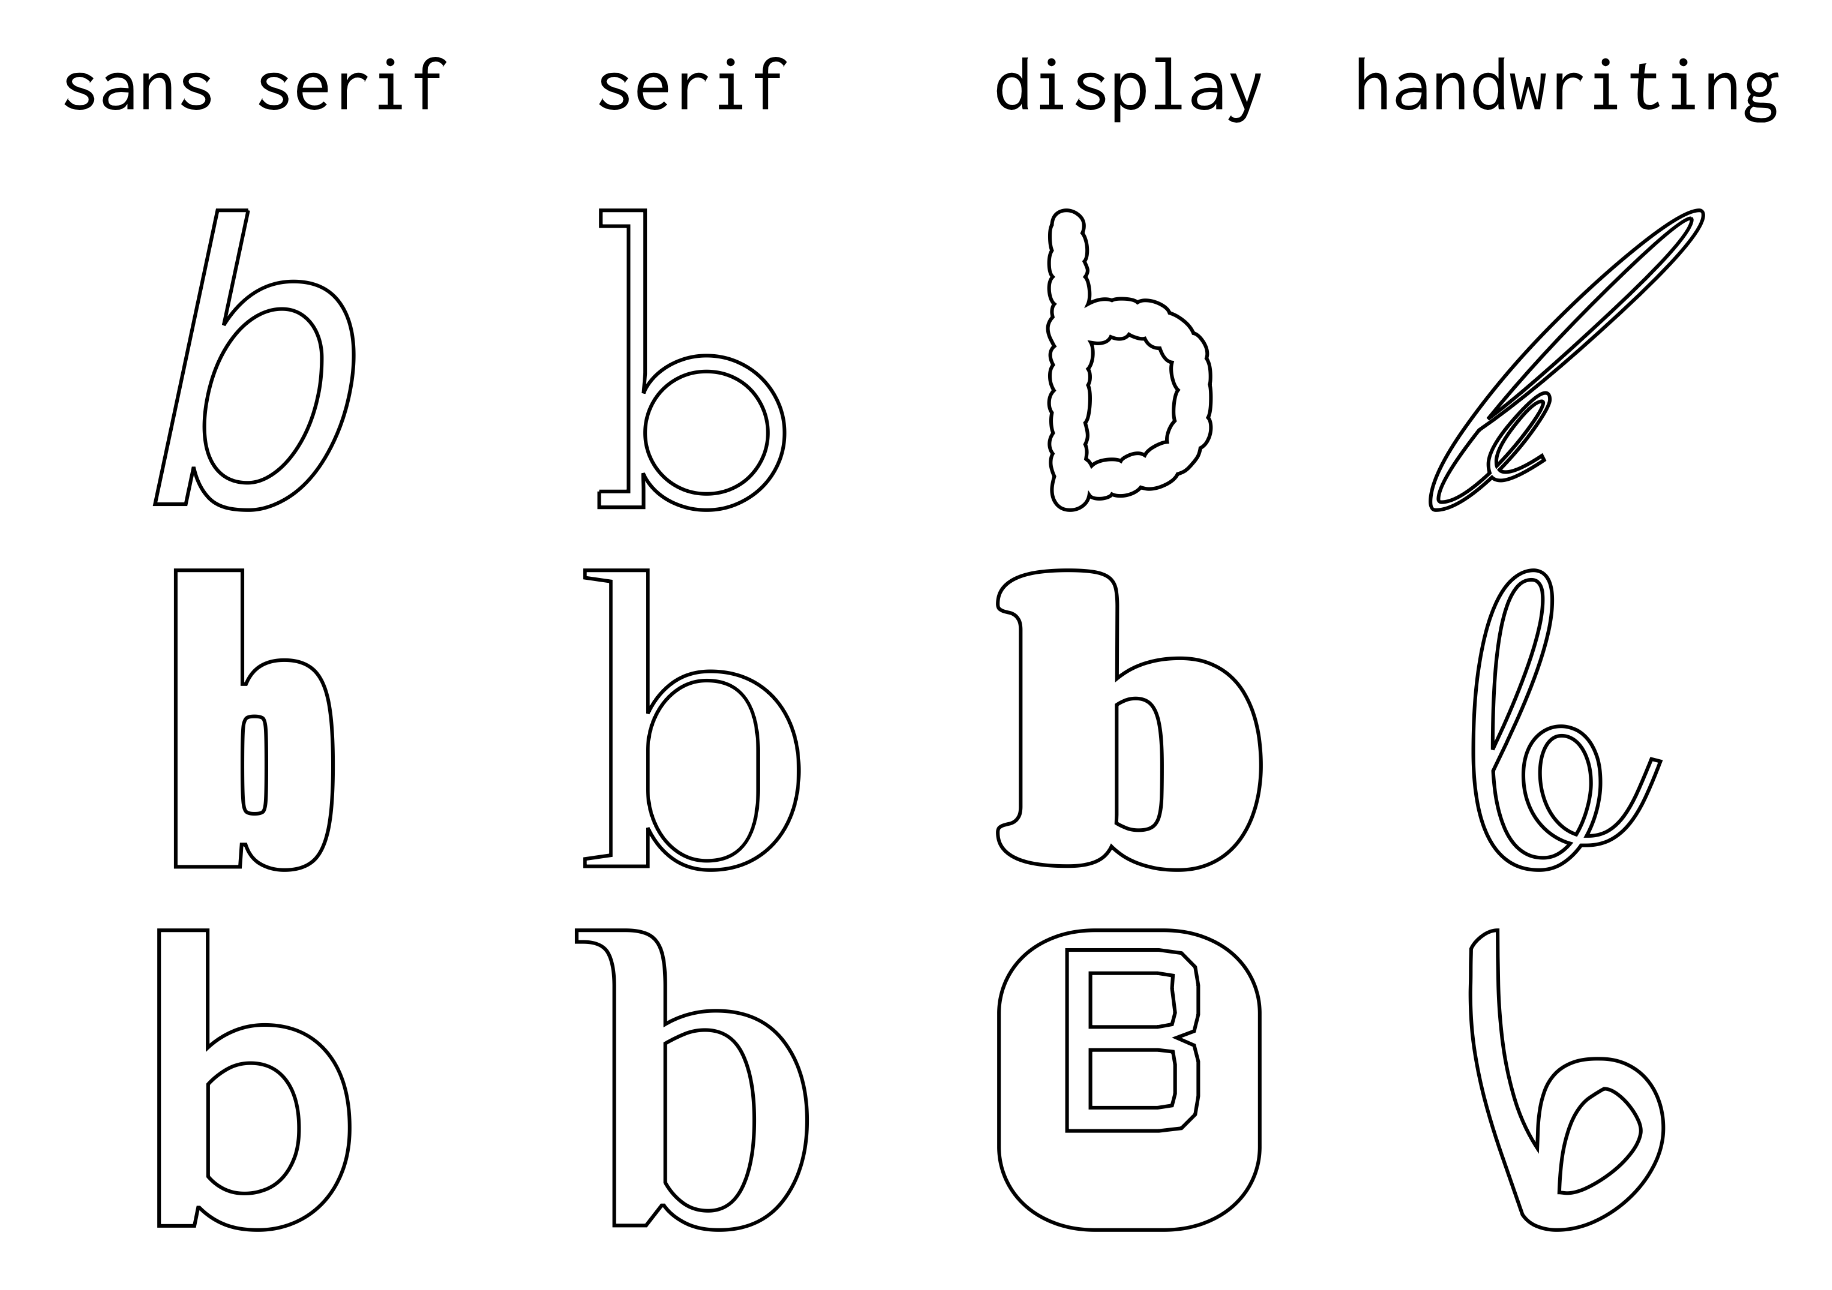
\includegraphics[width=0.55\textwidth]{figures/font_exs}
    \caption[Examples of glyphs from each font type]
    {Examples of glyphs from each font type. Serif glyphs have \textit{serifs}, or slight extensions off the ends of strokes, while sans serif glyphs do not.\label{fig:fonttypes}}
\end{figure}

In the context of computational modeling and generation, font glyphs offer certain advantages and pose distinctive challenges when compared to other types of designed graphics.
Unlike more complicated designs such as infographics and diagrams, they can be represented as drawings composed of simple lines and curves and, as such, can be modeled using sequential drawing commands.
However, font glyphs have distinct classes (i.e.\ each letter, number, symbol, etc.\ is a different class) and thus designing a generation procedure that is able to create clearly defined instances of different classes presents a challenge, as generation has to operate under strict constraints.

In this work, our computational methods are applied to font faces downloaded from Google Fonts\footnote{Downloaded from \url{https://github.com/google/fonts}, a GitHub repository containing all fonts in the dataset.}.
In Figure~\ref{fig:input_fonts}, a sampling of glyphs from the Google Fonts dataset is shown.

\begin{figure}[t]
	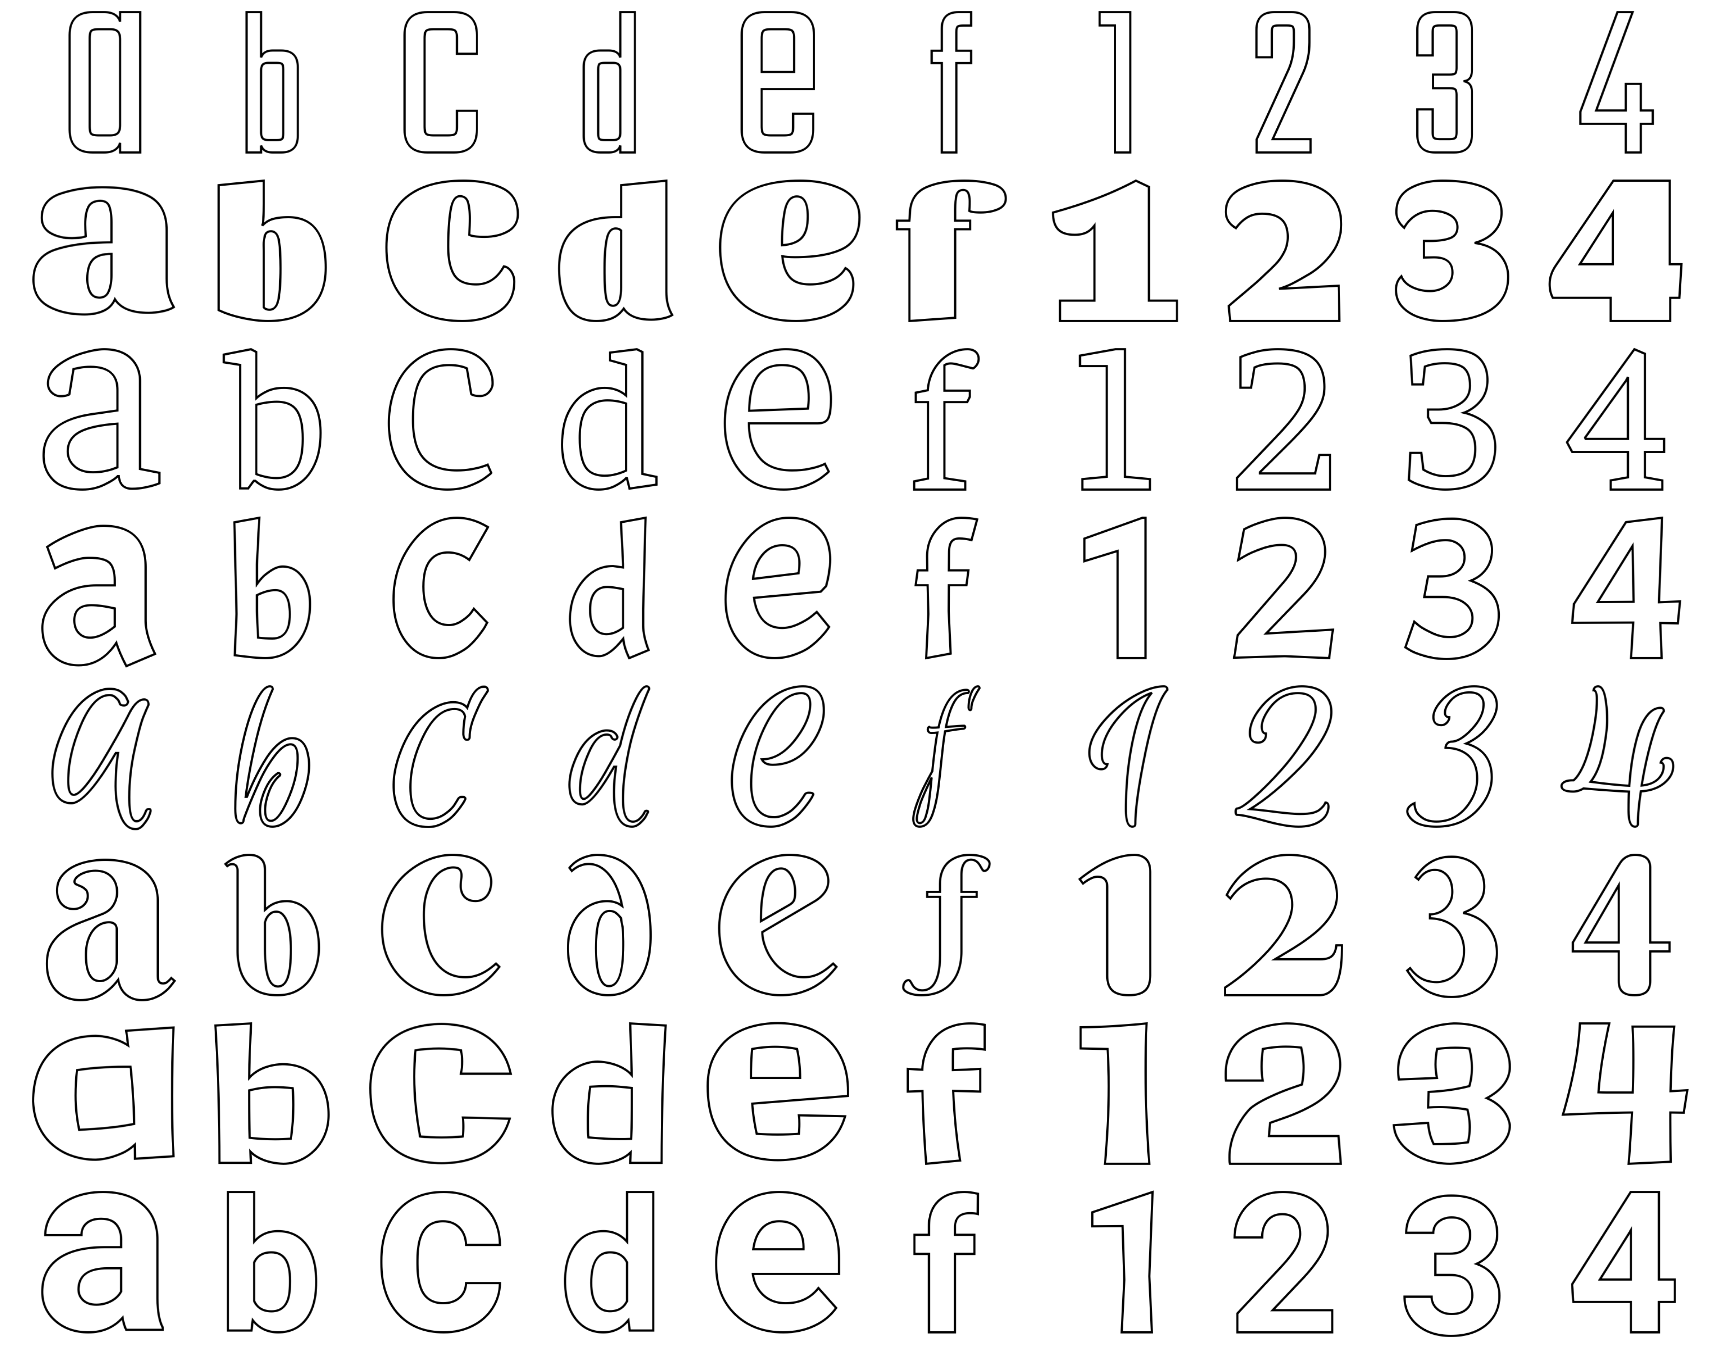
\includegraphics[width=\textwidth]{figures/input_fonts}
    \caption[A sample of the types of font faces used in our fonts dataset]{A sample of the types of font glyphs used in our dataset. Lowercase letters ``a'' through ``f'' are shown, as well as digits 1 through 4. Note the variety of styles represented: the dataset includes serif, sans serif, display, and handwriting style fonts.\label{fig:input_fonts}}
\end{figure}

\subsection{Vector graphics}
We are primarily interested in applying computational models to vector graphics as opposed to raster images.
While raster images encode color values for each point (or \textit{pixel}) in a two-dimensional grid, vector graphics describe a set of curves and shapes parameterized by mathematical equations and control points.
Many specifications exist for describing images in vector format, including SVG, Encapsulated PostScript (EPS), and Adobe PDF\@.
Font faces are often distributed as TrueType (TTF) files, which encode line and curve commands as well as metadata to aid with rendering.

Although the focus of our research is on font glyph inputs, our vision is to build a generalizable system for the variety of vector graphics generated by designers, including icons and logos.
Thus, our system accepts SVG data as input, as most vector graphics formats (including TTF) can be expressed using the commands available in the SVG specification.

\begin{figure}[t]
    \subcaptionbox{Raster images are defined as two-dimensional arrays of pixel values, while vector graphics define curves and paths mathematically. When scaled, vector graphics (right half) can still be rendered smoothly while raster images (left half) degrade in quality.\label{fig:svg-a}}
    {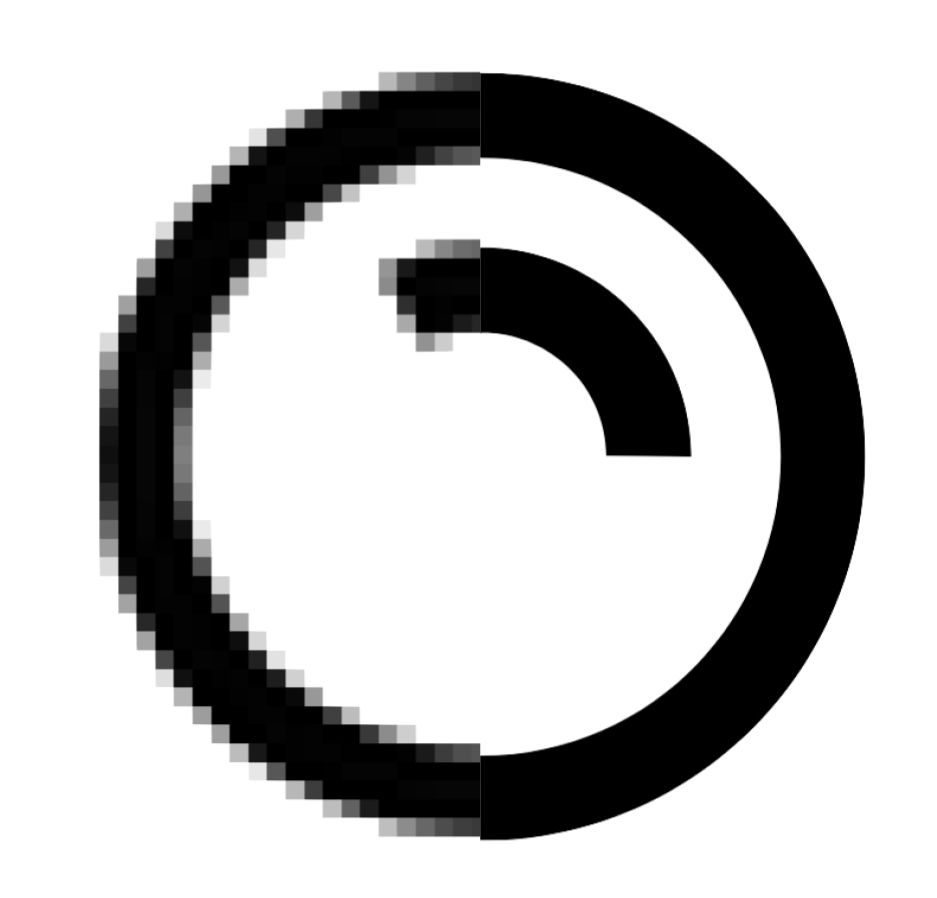
\includegraphics[height=1.85in]{figures/b_vs_vec}} \quad
    \subcaptionbox{SVG is an XML-based markup language that describes geometric elements within a vector image. A single path is used to draw this soap bubble, and colored curves in the image correspond approximately to the highlighted attribute commands that describe them. For example, the command \code{l-0.69-1.32} indicates a line drawn from a starting point to a point 0.69 units to the left and 1.32 units down.\label{fig:svg-b}}
    {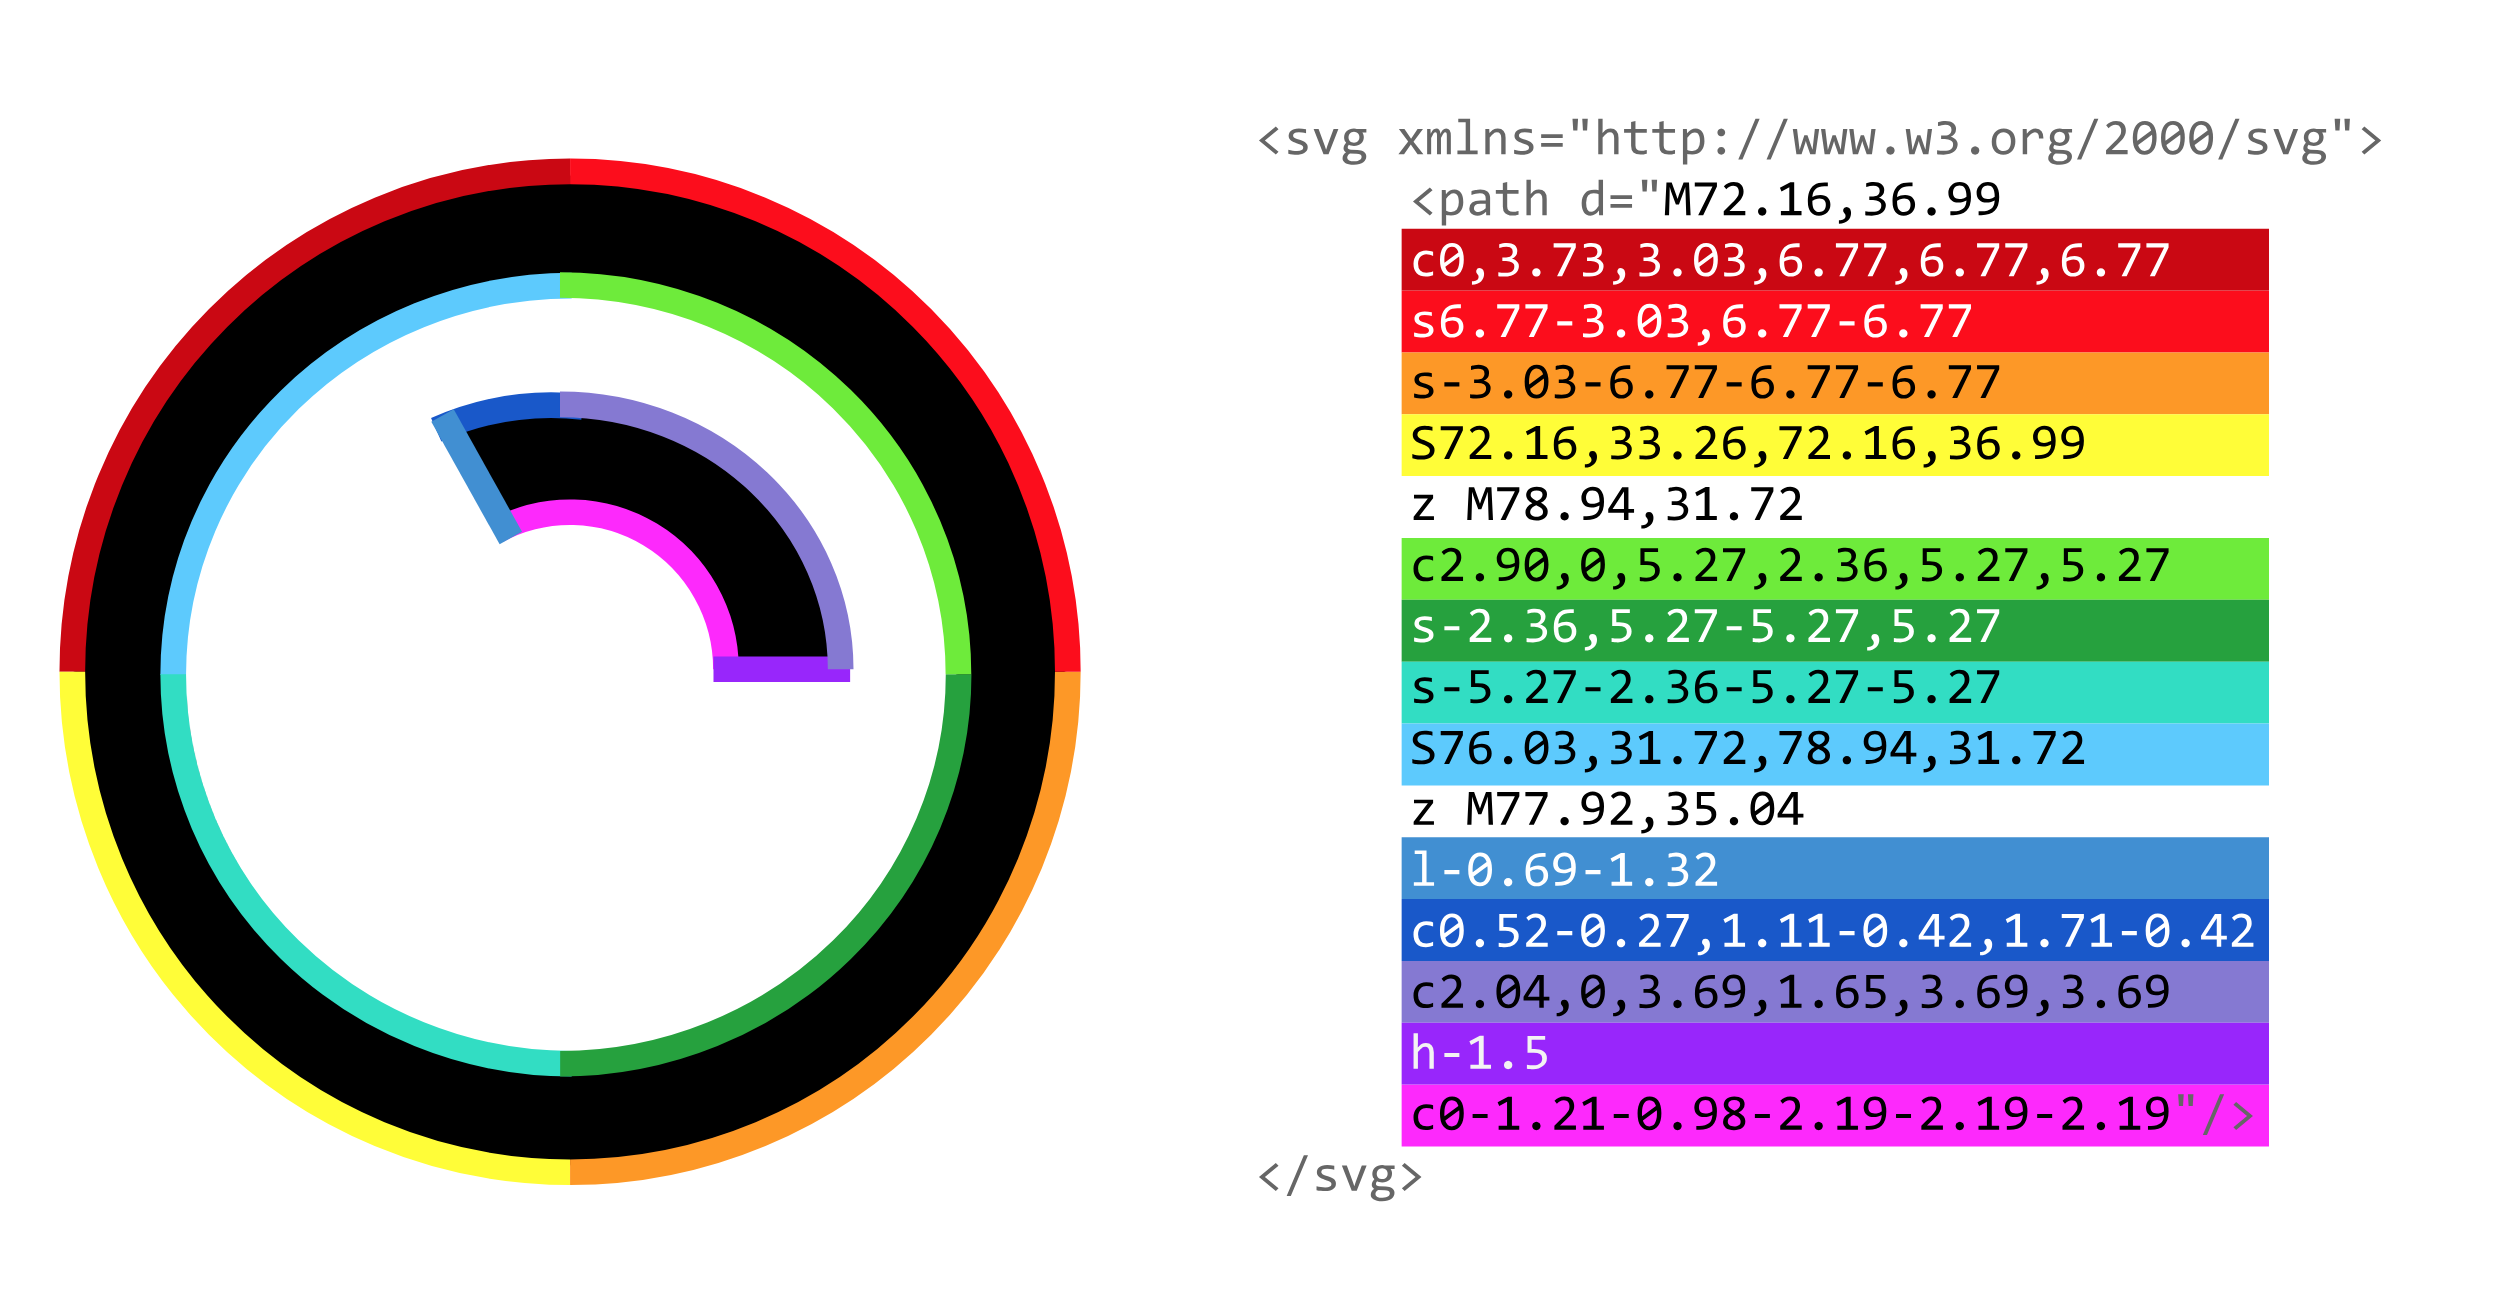
\includegraphics[height=1.85in]{figures/svgs}}
    \caption[An overview of vector graphics and Scalable Vector Graphics (SVG)]
    {A visual comparison of raster and vector graphics, and a sample SVG path.
    Image source: \textit{Dog Wash} by Llisole from the Noun Project.\label{fig:svg}}
\end{figure}

\subsubsection{Modeling vector graphics}
Applying computer vision techniques to vector graphics raises new challenges.
While bitmap and vector data can both decode into the same visual output, their underlying encoding structures have vast differences (Figure~\ref{fig:svg-a}).
As a data format, SVGs describe lists of geometric objects (among other elements such as text which are outside the scope of this work), including lines, circles, polygons, and splines.
The SVG \code{path} element, in particular, can be used to create all other element shapes.
Its attributes describe a series of commands that move from point to point, drawing curves or lines between them, as shown in Figure~\ref{fig:svg-b}.

The early popular deep convolutional network architectures designed to classify natural images, such as in~\cite{krizhevsky2012imagenet} and~\cite{simonyan2014very}, were designed to take in length $M\times N$ input vectors whose values directly represent corresponding pixel values in size $M\times N$ pixel input images.
While this model works well for raster images, this fixed-dimension format is incompatible with SVG element lists because their paths can describe any number of different point locations.
Instead, SVGs as sequential, variable-length, structured text are better suited to representation in models such as recurrent neural nets (RNNs).
RNNs are designed to model temporal sequences by unraveling across timesteps; long short-term memory (LSTM) models in particular use gated units to optimize for learning longer term dependencies~\cite{hochreiter1997long}.

\section{Generative modeling}
To solve the problem of creating novel vector drawings, we look towards the tools provided by generative machine learning methods.
While discriminative modeling techniques focus on separating and identifying inputs to produce output labels learned from high-dimensional data such as images, generative algorithms create previously unseen instances of a class based on representative inputs.
They are trained in an unsupervised or semi-supervised manner to learn a data distribution $P$, estimating the true data distribution $P_{gt}$ from which samples are drawn.
By drawing probabilistically from $P$, they can then be used to synthesize novel, unseen examples similar to input data.

Popular neural network-based approaches include generative-adversarial networks (GANs)~\cite{karpathy2016generative} and variational autoencoders (VAEs).
Introduced in~\citeyear{goodfellow2014generative}~\cite{goodfellow2014generative}, GANs pit a generative model $G(z; \theta_g)$ against an adversary $D(x; \theta_d)$ that learns to discriminate between samples from the ground truth dataset and the generative model's latent space.
When both $G$ and $D$ model differentiable functions, backpropagation can be used to train them towards convergence in a computationally efficient manner.

\subsection{Variational autoencoders}
Variational autoencoders, introduced in~\cite{kingma2013auto}, learn an encoder function mapping training examples from the input space $\mathcal{X}$ to vectors $z$ in the latent space $\mathcal{Z}$, as well as a decoder function that takes $z$ vectors sampled from a probability distribution $P(z)$ and applies a function that produces a random vector in the space $\mathcal{X}$~\cite{doersch2016tutorial}.
Intuitively, the goal is to train the model to produce outputs that look similar to the $x$ inputs but can be generated with some random noise such that they are distinct from training inputs.
To accomplish this goal, training a VAE tunes parameters $\theta$ to maximize the likelihood of reconstructing training examples after passing them through the entire pipeline, since increasing the probability of recreating $x$ inputs also increases the probability of creating similar random outputs.
Formally, we aim to maximize

\begin{equation}
    P(x) = \int P(x|\theta; z) P(z) dz
\end{equation}

Often, $P(x|\theta; z) = \mathcal{N}(x|f(\theta; z), \sigma^2 *I)$ where $\sigma$ is a parameter that can be set to manipulate the divergence of the generated output from training examples. In training, we constrain $P(z) = \mathcal{N}(0, 1)$ to simplify the loss calculation. 

Transforming this objective function to be differentiable and thus trainable using stochastic gradient descent requires a key insight: instead of sampling many $z_i$ then averaging $P(x|z_i)$, we focus only on the $z$ values that are likely to produce $x$ and compute $P(x)$ from those.
Our encoder then learns $Q(z|x; \phi)$ that approximates $P(z|x)$, while the decoder learns $P(x|z; \theta)$.
We can then define a loss function that describes a variational lower bound, where Kullback-Leibler (KL) divergence $\mathcal{D}$ accounts for the similarity between our $Q(z|x; \phi)$ and the true $P(z)$ and the reconstruction loss accounts for similarity between input and output:

\begin{equation}
    \mathcal{L}_i = -E_{z\sim Q(z|x_i; \phi)} [\log P(x_i|z; \theta)] + \mathcal{D}(Q(z|x_i; \phi)||P(z))
\end{equation}

In~\cite{graves2013generating}, the reconstruction loss function is expanded to account for sequential inputs and outputs, combining log loss for each item in the sequence.
This adjusted reconstruction loss can be used in a recurrent VAE architecture, where encoders and decoders digest sequential data.

\section{Related work}
Our end-to-end SVG generation model is inspired by prior work in line drawing generation, as both domains share an underlying temporal data structure.
Furthermore, our application to font generation is preceded by a history of computational approaches to font parameterization and style classification.

\subsection{Generating drawings}
Unconditionally generating parameterized curves extends the established problem of polyline generation.
Thus, we look towards contributions in handwriting and sketch generation, such as \citeauthor{graves2013generating}'s RNN-based handwriting prediction and synthesis work~\cite{graves2013generating}.
DRAW, a system introduced in~\cite{gregor2015draw}, uses a pair of recurrent networks in an VAE architecture to model attention in MNIST character generation.
Recent work by \citeauthor{ganin2017synthesizing} uses a reinforcement learning approach to train an agent to draw sketches~\cite{ganin2017synthesizing}.

Polyline results can easily be vectorized to produce splines, as in~\cite{janssen1997adaptive} or~\cite{birdal2014novel}.
However, our approach aims to model the entire SVG input to directly produce ready-to-edit spline output.
In our work, we build upon the variational autoencoder method presented by~\citeauthor{ha2017neural} in~\cite{ha2017neural}.
We use a similar bidirectional sequence-to-sequence VAE, with an overall loss calculation that includes drawing location losses, pen state losses, and KL loss.

\subsection{Font style}
\citeauthor{knuth1979tex}'s Metafont format demonstrates pioneering work in font style parameterization and has since motivated high-level font classification systems with font faces parameterized by human-controlled features like curvature and stroke width~\cite{knuth1979tex}\cite{lau2009learning}\cite{hassan2010next}.

Outside of manual feature selection approaches, many existing methods for modeling font style use font glyph raster images.
Tenenbaum and Freeman present a method for modeling style and content separately and apply it to font style extrapolation~\cite{tenenbaum1997separating}.
In~\cite{campbell2014learning}, polyline outlines are used to match glyphs across fonts using an energy optimization process, resulting in a learned manifold of fonts from which novel styles can be sampled.
Approaches for learning stylized calligraphy, such as~\cite{xu2005automatic}, take a more procedural approach, where strokes within characters are first extracted using shape segmentation approaches before use in training.
Neural network and VAE techniques to learning font style are increasingly common, such as in~\cite{upchurch2016z} and~\cite{wang2015deepfont}, and \citeauthor{lian2016automatic} use a combination of stroke segmentation and feature learning to generate handwriting fonts for Chinese characters~\cite{lian2016automatic}.

\appendix
\chapter{Arc conversion}\label{app:algs}
Our method for approximating SVG arc segments with cubic B\'ezier curves is as follows:
\begin{enumerate}
    \item Extract the arc parameters: start coordinates, end coordinates, ellipse major and minor radii, rotation angle from $x$ and $y$ axes, large arc flag, and sweep flag. 
    \item Transform ellipse into unit circle by rotating, scaling, and translating, and save those transformation factors.
    \item Find the arc angle from the transformed start point to end point on the unit circle.
    \item If needed, split the arc into segments, each covering an angle less than $90^\circ$.
    \item Approximate each segment angle's arc on a unit circle such that the distance from the circle center to the arc along the angle bisector of the arc is equal to the radius, defining cubic B\'ezier control points.
	\item Invert the transformation above to convert arcs along the unit circle back to the elliptical arc, transforming the generated control points accordingly.
	\item Use these transformed control points to parameterize the output cubic B\'ezier curve.
\end{enumerate}

\chapter{Dataset statistics}\label{app:data}
\begin{figure}[h]
\caption[Dataset statistics for other glyphs]
{Dataset statistics for the remaining glyphs on which our model was trained across all 2552 font faces in the Google Fonts dataset.\label{fig:stats-rem}}
\centering
\subcaptionbox*{}
{\begin{tikzpicture}
\begin{axis}[
 	xlabel={feature vector count},
	ylabel={number of ``f'' glyphs},
	width=0.45\textwidth,
    ybar,
    ymin=0
]
\addplot [
	fill=color1,
	fill opacity=0.4,
    hist={
        bins=7,
        data min=0.5,
        data max=300
    }   
] table [y index=0] {data/f_points_stats.csv};
\end{axis}
\end{tikzpicture}
}
\subcaptionbox*{}
{\begin{tikzpicture}
\begin{axis}[
 	xlabel={command type count},
	ylabel={number of ``f'' glyphs},
	width=0.45\textwidth,
    ybar,
    ymin=0
]
\addplot [
	fill=color2,
	fill opacity=0.4,
    hist={
        bins=7,
        data min=0.5,
        data max=100
    }   
] table [y index=0] {data/f_line_count.csv};
\addplot [
	fill=color3,
	fill opacity=0.4,
    hist={
        bins=7,
        data min=0.5,
        data max=100
    }   
] table [y index=0] {data/f_quad_count.csv};
\addlegendentry{\code{line}}
\addlegendentry{\code{quad}}
\end{axis}
\end{tikzpicture}
}

\subcaptionbox*{}
{\begin{tikzpicture}
\begin{axis}[
 	xlabel={feature vector count},
	ylabel={number of ``g'' glyphs},
	width=0.45\textwidth,
    ybar,
    ymin=0
]
\addplot [
	fill=color1,
	fill opacity=0.4,
    hist={
        bins=7,
        data min=0.5,
        data max=300
    }   
] table [y index=0] {data/g_points_stats.csv};
\end{axis}
\end{tikzpicture}
}
\subcaptionbox*{}
{\begin{tikzpicture}
\begin{axis}[
 	xlabel={command type count},
	ylabel={number of ``g'' glyphs},
	width=0.45\textwidth,
    ybar,
    ymin=0
]
\addplot [
	fill=color2,
	fill opacity=0.4,
    hist={
        bins=7,
        data min=0.5,
        data max=100
    }   
] table [y index=0] {data/g_line_count.csv};
\addplot [
	fill=color3,
	fill opacity=0.4,
    hist={
        bins=7,
        data min=0.5,
        data max=100
    }   
] table [y index=0] {data/g_quad_count.csv};
\addlegendentry{\code{line}}
\addlegendentry{\code{quad}}
\end{axis}
\end{tikzpicture}
}
\end{figure}

\begin{figure}[h]
\centering
\subcaptionbox*{}
{\begin{tikzpicture}
\begin{axis}[
 	xlabel={feature vector count},
	ylabel={number of ``o'' glyphs},
	width=0.45\textwidth,
    ybar,
    ymin=0
]
\addplot [
	fill=color1,
	fill opacity=0.4,
    hist={
        bins=7,
        data min=0.5,
        data max=300
    }   
] table [y index=0] {data/o_points_stats.csv};
\end{axis}
\end{tikzpicture}
}
\subcaptionbox*{}
{\begin{tikzpicture}
\begin{axis}[
 	xlabel={command type count},
	ylabel={number of ``o'' glyphs},
	width=0.45\textwidth,
    ybar,
    ymin=0
]
\addplot [
	fill=color2,
	fill opacity=0.4,
    hist={
        bins=7,
        data min=0.5,
        data max=100
    }   
] table [y index=0] {data/o_line_count.csv};
\addplot [
	fill=color3,
	fill opacity=0.4,
    hist={
        bins=7,
        data min=0.5,
        data max=100
    }   
] table [y index=0] {data/o_quad_count.csv};
\addlegendentry{\code{line}}
\addlegendentry{\code{quad}}
\end{axis}
\end{tikzpicture}
}

\subcaptionbox*{}
{\begin{tikzpicture}
\begin{axis}[
 	xlabel={feature vector count},
	ylabel={number of ``x'' glyphs},
	width=0.45\textwidth,
    ybar,
    ymin=0
]
\addplot [
	fill=color1,
	fill opacity=0.4,
    hist={
        bins=7,
        data min=0.5,
        data max=300
    }   
] table [y index=0] {data/x_points_stats.csv};
\end{axis}
\end{tikzpicture}
}
\subcaptionbox*{}
{\begin{tikzpicture}
\begin{axis}[
 	xlabel={command type count},
	ylabel={number of ``x'' glyphs},
	width=0.45\textwidth,
    ybar,
    ymin=0
]
\addplot [
	fill=color2,
	fill opacity=0.4,
    hist={
        bins=7,
        data min=0.5,
        data max=100
    }   
] table [y index=0] {data/x_line_count.csv};
\addplot [
	fill=color3,
	fill opacity=0.4,
    hist={
        bins=7,
        data min=0.5,
        data max=100
    }   
] table [y index=0] {data/x_quad_count.csv};
\addlegendentry{\code{line}}
\addlegendentry{\code{quad}}
\end{axis}
\end{tikzpicture}
}

\subcaptionbox*{}
{\begin{tikzpicture}
\begin{axis}[
 	xlabel={feature vector count},
	ylabel={number of ``0'' glyphs},
	width=0.45\textwidth,
    ybar,
    ymin=0
]
\addplot [
	fill=color1,
	fill opacity=0.4,
    hist={
        bins=7,
        data min=0.5,
        data max=300
    }   
] table [y index=0] {data/zero_points_stats.csv};
\end{axis}
\end{tikzpicture}
}
\subcaptionbox*{}
{\begin{tikzpicture}
\begin{axis}[
 	xlabel={command type count},
	ylabel={number of ``0'' glyphs},
	width=0.45\textwidth,
    ybar,
    ymin=0
]
\addplot [
	fill=color2,
	fill opacity=0.4,
    hist={
        bins=7,
        data min=0.5,
        data max=100
    }   
] table [y index=0] {data/zero_line_count.csv};
\addplot [
	fill=color3,
	fill opacity=0.4,
    hist={
        bins=7,
        data min=0.5,
        data max=100
    }   
] table [y index=0] {data/zero_quad_count.csv};
\addlegendentry{\code{line}}
\addlegendentry{\code{quad}}
\end{axis}
\end{tikzpicture}
}
\end{figure}

\begin{figure}[h]
\centering
\subcaptionbox*{}
{\begin{tikzpicture}
\begin{axis}[
 	xlabel={feature vector count},
	ylabel={number of ``1'' glyphs},
	width=0.45\textwidth,
    ybar,
    ymin=0
]
\addplot [
	fill=color1,
	fill opacity=0.4,
    hist={
        bins=7,
        data min=0.5,
        data max=300
    }   
] table [y index=0] {data/one_points_stats.csv};
\end{axis}
\end{tikzpicture}
}
\subcaptionbox*{}
{\begin{tikzpicture}
\begin{axis}[
 	xlabel={command type count},
	ylabel={number of ``1'' glyphs},
	width=0.45\textwidth,
    ybar,
    ymin=0
]
\addplot [
	fill=color2,
	fill opacity=0.4,
    hist={
        bins=7,
        data min=0.5,
        data max=100
    }   
] table [y index=0] {data/one_line_count.csv};
\addplot [
	fill=color3,
	fill opacity=0.4,
    hist={
        bins=7,
        data min=0.5,
        data max=100
    }   
] table [y index=0] {data/one_quad_count.csv};
\addlegendentry{\code{line}}
\addlegendentry{\code{quad}}
\end{axis}
\end{tikzpicture}
}

\subcaptionbox*{}
{\begin{tikzpicture}
\begin{axis}[
 	xlabel={feature vector count},
	ylabel={number of ``2'' glyphs},
	width=0.45\textwidth,
    ybar,
    ymin=0
]
\addplot [
	fill=color1,
	fill opacity=0.4,
    hist={
        bins=7,
        data min=0.5,
        data max=300
    }   
] table [y index=0] {data/two_points_stats.csv};
\end{axis}
\end{tikzpicture}
}
\subcaptionbox*{}
{\begin{tikzpicture}
\begin{axis}[
 	xlabel={command type count},
	ylabel={number of ``2'' glyphs},
	width=0.45\textwidth,
    ybar,
    ymin=0
]
\addplot [
	fill=color2,
	fill opacity=0.4,
    hist={
        bins=7,
        data min=0.5,
        data max=100
    }   
] table [y index=0] {data/two_line_count.csv};
\addplot [
	fill=color3,
	fill opacity=0.4,
    hist={
        bins=7,
        data min=0.5,
        data max=100
    }   
] table [y index=0] {data/two_quad_count.csv};
\addlegendentry{\code{line}}
\addlegendentry{\code{quad}}
\end{axis}
\end{tikzpicture}
}

\subcaptionbox*{}
{\begin{tikzpicture}
\begin{axis}[
 	xlabel={feature vector count},
	ylabel={number of ``3'' glyphs},
	width=0.45\textwidth,
    ybar,
    ymin=0
]
\addplot [
	fill=color1,
	fill opacity=0.4,
    hist={
        bins=7,
        data min=0.5,
        data max=300
    }   
] table [y index=0] {data/three_points_stats.csv};
\end{axis}
\end{tikzpicture}
}
\subcaptionbox*{}
{\begin{tikzpicture}
\begin{axis}[
 	xlabel={command type count},
	ylabel={number of ``3'' glyphs},
	width=0.45\textwidth,
    ybar,
    ymin=0
]
\addplot [
	fill=color2,
	fill opacity=0.4,
    hist={
        bins=7,
        data min=0.5,
        data max=100
    }   
] table [y index=0] {data/three_line_count.csv};
\addplot [
	fill=color3,
	fill opacity=0.4,
    hist={
        bins=7,
        data min=0.5,
        data max=100
    }   
] table [y index=0] {data/three_quad_count.csv};
\addlegendentry{\code{line}}
\addlegendentry{\code{quad}}
\end{axis}
\end{tikzpicture}
}
\end{figure}

\begin{figure}[h]
\centering
\subcaptionbox*{}
{\begin{tikzpicture}
\begin{axis}[
 	xlabel={feature vector count},
	ylabel={number of ``4'' glyphs},
	width=0.45\textwidth,
    ybar,
    ymin=0
]
\addplot [
	fill=color1,
	fill opacity=0.4,
    hist={
        bins=7,
        data min=0.5,
        data max=300
    }   
] table [y index=0] {data/four_points_stats.csv};
\end{axis}
\end{tikzpicture}
}
\subcaptionbox*{}
{\begin{tikzpicture}
\begin{axis}[
 	xlabel={command type count},
	ylabel={number of ``4'' glyphs},
	width=0.45\textwidth,
    ybar,
    ymin=0
]
\addplot [
	fill=color2,
	fill opacity=0.4,
    hist={
        bins=7,
        data min=0.5,
        data max=100
    }   
] table [y index=0] {data/four_line_count.csv};
\addplot [
	fill=color3,
	fill opacity=0.4,
    hist={
        bins=7,
        data min=0.5,
        data max=100
    }   
] table [y index=0] {data/four_quad_count.csv};
\addlegendentry{\code{line}}
\addlegendentry{\code{quad}}
\end{axis}
\end{tikzpicture}
}

\subcaptionbox*{}
{\begin{tikzpicture}
\begin{axis}[
 	xlabel={feature vector count},
	ylabel={number of ``5'' glyphs},
	width=0.45\textwidth,
    ybar,
    ymin=0
]
\addplot [
	fill=color1,
	fill opacity=0.4,
    hist={
        bins=7,
        data min=0.5,
        data max=300
    }   
] table [y index=0] {data/five_points_stats.csv};
\end{axis}
\end{tikzpicture}
}
\subcaptionbox*{}
{\begin{tikzpicture}
\begin{axis}[
 	xlabel={command type count},
	ylabel={number of ``5'' glyphs},
	width=0.45\textwidth,
    ybar,
    ymin=0
]
\addplot [
	fill=color2,
	fill opacity=0.4,
    hist={
        bins=7,
        data min=0.5,
        data max=100
    }   
] table [y index=0] {data/five_line_count.csv};
\addplot [
	fill=color3,
	fill opacity=0.4,
    hist={
        bins=7,
        data min=0.5,
        data max=100
    }   
] table [y index=0] {data/five_quad_count.csv};
\addlegendentry{\code{line}}
\addlegendentry{\code{quad}}
\end{axis}
\end{tikzpicture}
}

\subcaptionbox*{}
{\begin{tikzpicture}
\begin{axis}[
 	xlabel={feature vector count},
	ylabel={number of ``6'' glyphs},
	width=0.45\textwidth,
    ybar,
    ymin=0
]
\addplot [
	fill=color1,
	fill opacity=0.4,
    hist={
        bins=7,
        data min=0.5,
        data max=300
    }   
] table [y index=0] {data/six_points_stats.csv};
\end{axis}
\end{tikzpicture}
}
\subcaptionbox*{}
{\begin{tikzpicture}
\begin{axis}[
 	xlabel={command type count},
	ylabel={number of ``6'' glyphs},
	width=0.45\textwidth,
    ybar,
    ymin=0
]
\addplot [
	fill=color2,
	fill opacity=0.4,
    hist={
        bins=7,
        data min=0.5,
        data max=100
    }   
] table [y index=0] {data/six_line_count.csv};
\addplot [
	fill=color3,
	fill opacity=0.4,
    hist={
        bins=7,
        data min=0.5,
        data max=100
    }   
] table [y index=0] {data/six_quad_count.csv};
\addlegendentry{\code{line}}
\addlegendentry{\code{quad}}
\end{axis}
\end{tikzpicture}
}
\end{figure}

\begin{figure}[h]
\centering
\subcaptionbox*{}
{\begin{tikzpicture}
\begin{axis}[
 	xlabel={feature vector count},
	ylabel={number of ``7'' glyphs},
	width=0.45\textwidth,
    ybar,
    ymin=0
]
\addplot [
	fill=color1,
	fill opacity=0.4,
    hist={
        bins=7,
        data min=0.5,
        data max=300
    }   
] table [y index=0] {data/seven_points_stats.csv};
\end{axis}
\end{tikzpicture}
}
\subcaptionbox*{}
{\begin{tikzpicture}
\begin{axis}[
 	xlabel={command type count},
	ylabel={number of ``7'' glyphs},
	width=0.45\textwidth,
    ybar,
    ymin=0
]
\addplot [
	fill=color2,
	fill opacity=0.4,
    hist={
        bins=7,
        data min=0.5,
        data max=100
    }   
] table [y index=0] {data/seven_line_count.csv};
\addplot [
	fill=color3,
	fill opacity=0.4,
    hist={
        bins=7,
        data min=0.5,
        data max=100
    }   
] table [y index=0] {data/seven_quad_count.csv};
\addlegendentry{\code{line}}
\addlegendentry{\code{quad}}
\end{axis}
\end{tikzpicture}
}

\subcaptionbox*{}
{\begin{tikzpicture}
\begin{axis}[
 	xlabel={feature vector count},
	ylabel={number of ``8'' glyphs},
	width=0.45\textwidth,
    ybar,
    ymin=0
]
\addplot [
	fill=color1,
	fill opacity=0.4,
    hist={
        bins=7,
        data min=0.5,
        data max=300
    }   
] table [y index=0] {data/eight_points_stats.csv};
\end{axis}
\end{tikzpicture}
}
\subcaptionbox*{}
{\begin{tikzpicture}
\begin{axis}[
 	xlabel={command type count},
	ylabel={number of ``8'' glyphs},
	width=0.45\textwidth,
    ybar,
    ymin=0
]
\addplot [
	fill=color2,
	fill opacity=0.4,
    hist={
        bins=7,
        data min=0.5,
        data max=100
    }   
] table [y index=0] {data/eight_line_count.csv};
\addplot [
	fill=color3,
	fill opacity=0.4,
    hist={
        bins=7,
        data min=0.5,
        data max=100
    }   
] table [y index=0] {data/eight_quad_count.csv};
\addlegendentry{\code{line}}
\addlegendentry{\code{quad}}
\end{axis}
\end{tikzpicture}
}

\subcaptionbox*{}
{\begin{tikzpicture}
\begin{axis}[
 	xlabel={feature vector count},
	ylabel={number of ``9'' glyphs},
	width=0.45\textwidth,
    ybar,
    ymin=0
]
\addplot [
	fill=color1,
	fill opacity=0.4,
    hist={
        bins=7,
        data min=0.5,
        data max=300
    }   
] table [y index=0] {data/nine_points_stats.csv};
\end{axis}
\end{tikzpicture}
}
\subcaptionbox*{}
{\begin{tikzpicture}
\begin{axis}[
 	xlabel={command type count},
	ylabel={number of ``9'' glyphs},
	width=0.45\textwidth,
    ybar,
    ymin=0
]
\addplot [
	fill=color2,
	fill opacity=0.4,
    hist={
        bins=7,
        data min=0.5,
        data max=100
    }   
] table [y index=0] {data/nine_line_count.csv};
\addplot [
	fill=color3,
	fill opacity=0.4,
    hist={
        bins=7,
        data min=0.5,
        data max=100
    }   
] table [y index=0] {data/nine_quad_count.csv};
\addlegendentry{\code{line}}
\addlegendentry{\code{quad}}
\end{axis}
\end{tikzpicture}
}
\end{figure}


%% This defines the bibliography file (main.bib) and the bibliography style.
%% If you want to create a bibliography file by hand, change the contents of
%% this file to a `thebibliography' environment.  For more information 
%% see section 4.3 of the LaTeX manual.
\begin{singlespace}
\bibliography{main}
\bibliographystyle{plain}
\end{singlespace}

\end{document}

